% !TEX root = ../my-thesis.tex
%
\chapter{Implementation}
\label{sec:implementation}
The approach of this thesis, described in the previous chapter, is realized as a reference implementation in the \textit{Python} programming language, which can be found here:~\url{https://github.com/Berberer/frankensteins-automl}.
For simplicity and practicability reasons, this implementation has some minor restrictions regarding the expected input, but this can be changed or generalized to more inputs with minor modifications.
As for the current implementation state, the optimization budget input is limited to time as the budget type and the dataset input has to be either in the \textit{ARFF} file format, popularized by \textit{WEKA}~\cite{Witten-Weka}, or directly as \textit{NumPy} arrays.

This reference implementation serves two different reason:
\begin{itemize}
	\item Help for a better understanding as an alternative and more practical representation of the approach, since it can be easier to read structured code instead of a theoretical and lengthy formal definition.
	\item For the evaluation of this approach and the comparison against other approaches and some baseline values in chapter~\ref{sec:evaluation}, this approach must be provided as an executable program to get results for different experimental settings.
\end{itemize}

The implementation is explained in the following chapter, which is structured into three parts.
At first, the architectural composition of the implementation and the interaction of the included components is explained.
With this overall perspective of the implementation, the codebase will be easier to understand and to navigate.
Since the implementation was not done from scratch, the utilized Python libraries are listed and their functionality explained as a second part to pay respect to their creators as well as elucidate their contribution to the overall functionality.
Finally, the description schema of the AutoML optimization space definition is provided, which is a required input for the implementation, such that a user can understand the included optimization spaces of the implementation and modify them if needed.

\section{Components of the Project and their Interaction}
\label{sec:implementation:components}
The components of the implementation and their architectural composition can be separated into three parts with regard to the subject matter and this separation will be used in the following to outline and explain the implementation.
All explanations of the implementation will be accompanied by UML class diagrams of the corresponding sources to support the description of the functionality.
These diagrams only depict the relevant core mechanics of the respective classes, while getter and setter methods as well as minor utility methods are omitted.\newline 
For the model selection as the first of the three components, the search space needs to be constructed from the input optimization space definition.
At first the components for this part of the implementation are explained.
In the second part, the components for evaluating machine learning pipelines and handling the different optimizers are explicated.
All components from this two parts are combined via a MCTS implementation into a overall AutoML program and all components for this are explained in the third part.

\subsection{Model Selection Search Space Management}
\label{sec:implementation:components:search-space}
Since the model selection is reduced to a graph search problem, the search space is managed as a graph as shown in~\ref{fig:implementation:uml:search-space}.
Because in other components basic graph modelling functionality is needed as well, abstract base classes for graph nodes and a graph generator are created.
Each \texttt{GraphNode} is identified by a unique id and knows its predecessor nodes as well as the successor nodes.
Depending on the use-case for the graph node, the abstract method \texttt{is\_leaf\_node} has to be implemented with the respected logic of the use-case.\newline
The associated \texttt{GraphGenerator} class has abstract methods for \texttt{get\_root\_node} and \texttt{get\_node\_successors}, which have to be implemented domain-specific as well.
Nevertheless, \texttt{get\_node\_successors} is not intended for general usage in other classes.
Instead, the method \texttt{generate\_successors} shall be used.
It performs checks if the parameter node is either a leaf node or already has a reference to its successor nodes.
Only if neither is the case, the abstract method \texttt{get\_node\_successors} is used to get new successors from scratch with the use-case specific logic.

For this specific case of having a HTN planning graph for model selection, the \texttt{SearchSpace}, \texttt{SearchSpaceComponent} and \texttt{SearchSpaceRestProblem} classes are the underlying data structure for modelling the HTN planning problem.\newline
Basically, \texttt{SearchSpaceComponent} is a wrapper class for components of the AutoML search space definition, which are given as input in a schema defined in~\ref{sec:implementation:json}.
Additionally, this class has some helper methods for handling parameters.
It can create the default parametrization or alternatively draw a random parametrization of this component.
For a given parametrization, it can check the validity, i.e. exists a value for each parameter and are all values valid for the corresponding parameter.
And finally, it can split a given parametrization into positional and keyword parameter for utilizing them for a concrete Python function call.\newline
With the \texttt{SearchSpace} class, all components defined in the input are managed and can accessed either by their name of by an interface they provide.\newline
Each step in a HTN planning process has a rest problem, i.e. which interfaces are satisfied and which are open.
The corresponding \texttt{SearchSpaceRestProblem} is utilized to store this information.
It saves all required interfaces that are present in the current plan and if they are already satisfied.
Additionally is has a mapping, which satisfied required interface is satisfied with which component that provides this interface.
For using this problem representation for a graph search, it has the methods \texttt{is\_satisfied}, which returns true if all required interfaces have a suitable mapped provided interface, and \texttt{get\_first\_unsatisfied\_required\_interface} to pick the next interface for progressing the planning.
Each graph node for the HTN planning graph represents, that one interface has been satisfied and therefore the class has an additional static method \texttt{from\_previous\_rest\_problem} to create a rest problem from another one by satisfying one required interface.

When all required interfaces of the considered HTN task tree are satisfied and a parametrization is generated, a concrete \texttt{SearchSpaceComponentInstance} can be created for a \texttt{SearchSpaceComponent} with this interface to component mapping and the parametrization.
With the method \texttt{construct\_pipeline\_element}, the actual pipeline element which is represented by the component can be instantiated and configured with the parameters and if necessary the pipeline elements of required interfaces.

Finally, the \texttt{GraphNode} and \texttt{GraphGenerator} classes are inherited for the use-case of model selection HTN planning via a graph search with the \texttt{SearchSpaceGraphNode} and \texttt{SearchSpaceGraphGenerator} classes.
The abstract methods of the base classes are implemented in the following manner:
\begin{itemize}
    \item \texttt{GraphNode.is\_leaf\_node}: Each \texttt{SearchSpaceNode} represents one specific rest problem.
    This node can be considered a leaf node of the planning graph if the \texttt{SearchSpaceRestProblem.is\_satisfied} returns true.
    \item \texttt{GraphGenerator.get\_root\_node}: The \texttt{SearchSpaceGraphGenerator} has the name of the start component of the planning problem as an initial input.
    It can get the corresponding component from the \texttt{SearchSpace} instance, construct a \texttt{SearchSpaceRestProblem} for this initial component and create the root node with it.
    \item \texttt{GraphGenerator.get\_node\_successors}: The rest problem of the node, provided as a parameter of this method, will return one specific unsatisfied interface with its \texttt{get\_first\_unsatisfied\_required\_interface} method.
    By calling \texttt{SearchSpace.get\_components\_providing\_interface} with the name of this first unsatisfied interface, all suitable components are found and afterwards calling \texttt{SearchSpaceRestProblem.from\_previous\_rest\_problem} for each of this components, will generate the rest problems for the successor nodes.
\end{itemize}

\begin{figure}[ht!]
    \centering
    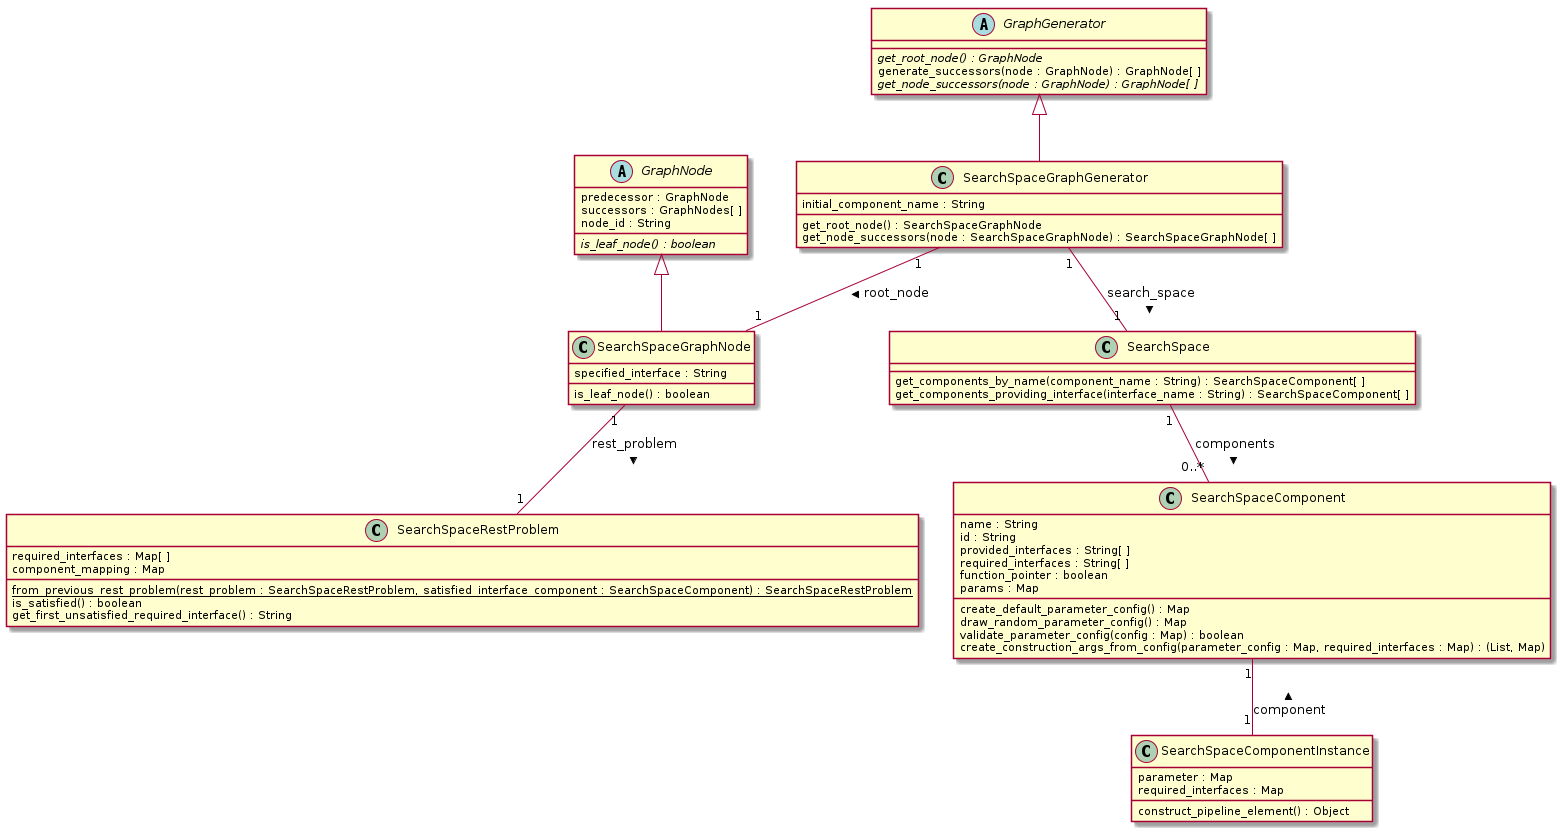
\includegraphics[angle=90,origin=c,width=\textwidth,height=0.7\textheight,keepaspectratio]{gfx/Figures/Implementation/search-space/SearchSpaceManagement.png}
    \caption{A simplified overview of the implementation components for managing the search space and enabling HTN planning in this space.}
    \label{fig:implementation:uml:search-space}
\end{figure}

\subsection{Pipeline Evaluation and Optimizers for Model Configuration}
\label{sec:implementation:components:optimization}
Once the model selection procedure has created a pipeline topology in the form of a satisfied \textit{SearchSpaceRestProblem}, the model configuration has to optimize a parametrization for the components of this topology.
This is the task of the optimizer ensembles, which are implemented as illustrated in~\ref{fig:implementation:uml:optimization}.\newline
For each created pipeline topology of the model selection, i.e. one for each Pipeline Node, one \texttt{OptimizationParameterDomain} object is created and attached.
It can manage the component and the corresponding parameter space of this pipeline as well as all already evaluated parametrization configuration.
The configurations are considered from two points of view: For creating actual pipeline objects for evaluation with a component mapping, where the parameters are stored in a map to have them associated to their component, and for optimizing this configurations, which is done in the more generalized form of NumPy arrays, i.e. basically vectors.
Between this two perspectives, the optimization domain \texttt{OptimizationParameterDomain} can perform transformations between both formats.\newline
As a starting point for optimization runs the domain can create the default configuration and random configurations.
Afterwards during the optimization, the domain keeps track of all results in both a heap as well as a mapping from a hashed parametrization id to the scores.
This duplicate storing has the downside of a higher memory consumption, but the upside of faster access in two different use-cases:
\begin{enumerate}
    \item Retrieving the top $n$ results from all already evaluated results via the heap, if one optimization method needs this for a warmstart.
    \item Checking if one found parametrization was already evaluated and if yes to retrieve the score to prevent a repeated evaluation via the map.
\end{enumerate}

The core functionality that each optimizer needs is provided in the \texttt{AbstractOptimizer} base class, which provides the following mechanics:
\begin{itemize}
    \item \texttt{\_score\_candidate}: Check in the domain, if the parametrization has already been evaluated and return this result if yes.
    Otherwise, utilize the attached \texttt{PipelineEvaluator} class to construct a pipeline from a satisfied rest problem, which is provided from the pipeline node, and evaluate the accuracy of the pipeline in a detached process for a better parallelization and add this new score to the domain.
    \item \texttt{\_random\_transform\_candidate}: Changes $n$ random elements of the candidate parametrization vector by a small random value.
    This is used for the search step in the random search and therewith Hyperband as well and the mutations of the Genetic Algorithm.
\end{itemize}
Each optimization algorithm now has to implement the abstract \texttt{perform\_optimization} method, which is given the optimization time budget as an input, to perform the corresponding optimization logic of this algorithm.

In this current reference implementation, five optimization algorithms are implemented:
\begin{itemize}
    \item \texttt{RandomSearch}: This random search implementation is based on the second variant from~\ref{sec:theory:optimization:search}, i.e. it warmstarts with the best candidate so far from the optimization domain of this pipeline topology, if one exists, as the current candidate and takes the default configuration as an alterative if no parametrization was evaluated yet.
    Afterwards, a random point from a small hypersphere surrounding the current candidate is selected and evaluated.
    If this newly selected candidate shows an improvement, it is selected as the next current candidate for the next search step iteration.
    Otherwise, the last current candidate is kept.
    This is repeated until the optimization budget is spent.
    \item \texttt{Hyperband}: This Hyperband implementation is based on an existing open-source implementation~\footnote{\url{https://github.com/zygmuntz/hyperband}}.
    The existing implementation is utilized in the \texttt{HyperbandRunner} class which is called by the \texttt{Hyperband} optimizer class as a part of the common integration concept via the \texttt{AbstractOptimizer} class.
    It is warmstarted by selecting the top 50 configurations from the optimization domain, or alternatively all existing if there are less then 50, and fill the list of starting points with random configurations up until 100 starting points for the Hyperband random searches.
    \item \texttt{GeneticAlgorithm}: For this reference implementation, the genetic algorithm implementation was modelled after \textit{TPOT}, since this approach has shown good results for tackling AutoML problems with genetic algorithms.
    Therefore, the following operations are applied to each produce the generation from an existing generation of 100 individuals:
        \begin{enumerate}
            \item Selected the top 20 individuals.
            \item Create 5 copies of each individual to get back to a population size of 100 for the next generation.
            \item Select 10 random offsprings out of this 100 offsprings and create 10 new offsprings out of them via one-point crossovers of random pairs of this 10.
            \item The remaining 90 candidates are modified in the form of point mutations.
        \end{enumerate}
    The warmstarted initial generation of 100 individuals for each genetic algorithm run is initiated similar to Hyperband, but with the exception of the best 20 configurations and 80 random configurations.
    \item \texttt{SMAC}: This is a wrapper class for the official \textit{SMAC} implementation.
    As in the Hyperband integration, it is warmstarted with the top 50 candidates, if so many exist, and additional random configurations to get 100 starting point configurations.
    \item \texttt{DiscretizationSearch}: This optimizer approach was inspired by \textit{ML-Plan}, but instead of creating a search graph for the complete AutoML problem solution space, it is here solely applied on hyperparameter optimization.
    In the optimization domain an order is set for the parameter of the pipeline topology and this order is also applied for creating the parameter value space for the discretizations.
    For parameters of type boolean or categorical, a single node is sufficient where each child node represents true or false, or alternatively each categorical value.
    In the case of integer or real numbers, the minimum and maximum can be really far apart and creating a child node with a high coverage of the values in between will blow up the degree of the graph enormously.
    Instead, numeric parameters are split by half and one child node is attached for each half until each half consists only of a single number in the case of integers, or the lower and upper bound of the halves are smaller then $\varepsilon \cdot (\max(p) - min(p))$ of the range of parameter $p$, in which case this node represents th value $\frac{\max(p) - min(p)}{2}$.\newline
    For creating this discretizations dependent on the type, the \textit{Discretization} class and especially its static methods are used.
    Once more, subclasses of \texttt{GraphNode} and \texttt{GraphGenerator} are created where each node represents one discretization down to the leaf nodes where, the the last parameter value is discretized as far as possible and therewith the actual value selected. 
    Here, the discretization is atomic.\newline
    The graph that is created with this mechanism is searched via a best-first search, where each node is scored via the best result of three Monte-Carlo simulations.
    If all child nodes of a node were visited during the search, this node is marked as \texttt{covered} and will be ignored from this point on.
    Hence, it can occur for small parameter spaces and large optimization budgets, that this approach fill finish before the optimization budget is spent because of the discretized view of a continuos space.
\end{itemize}

\begin{figure}[ht!]
    \centering
    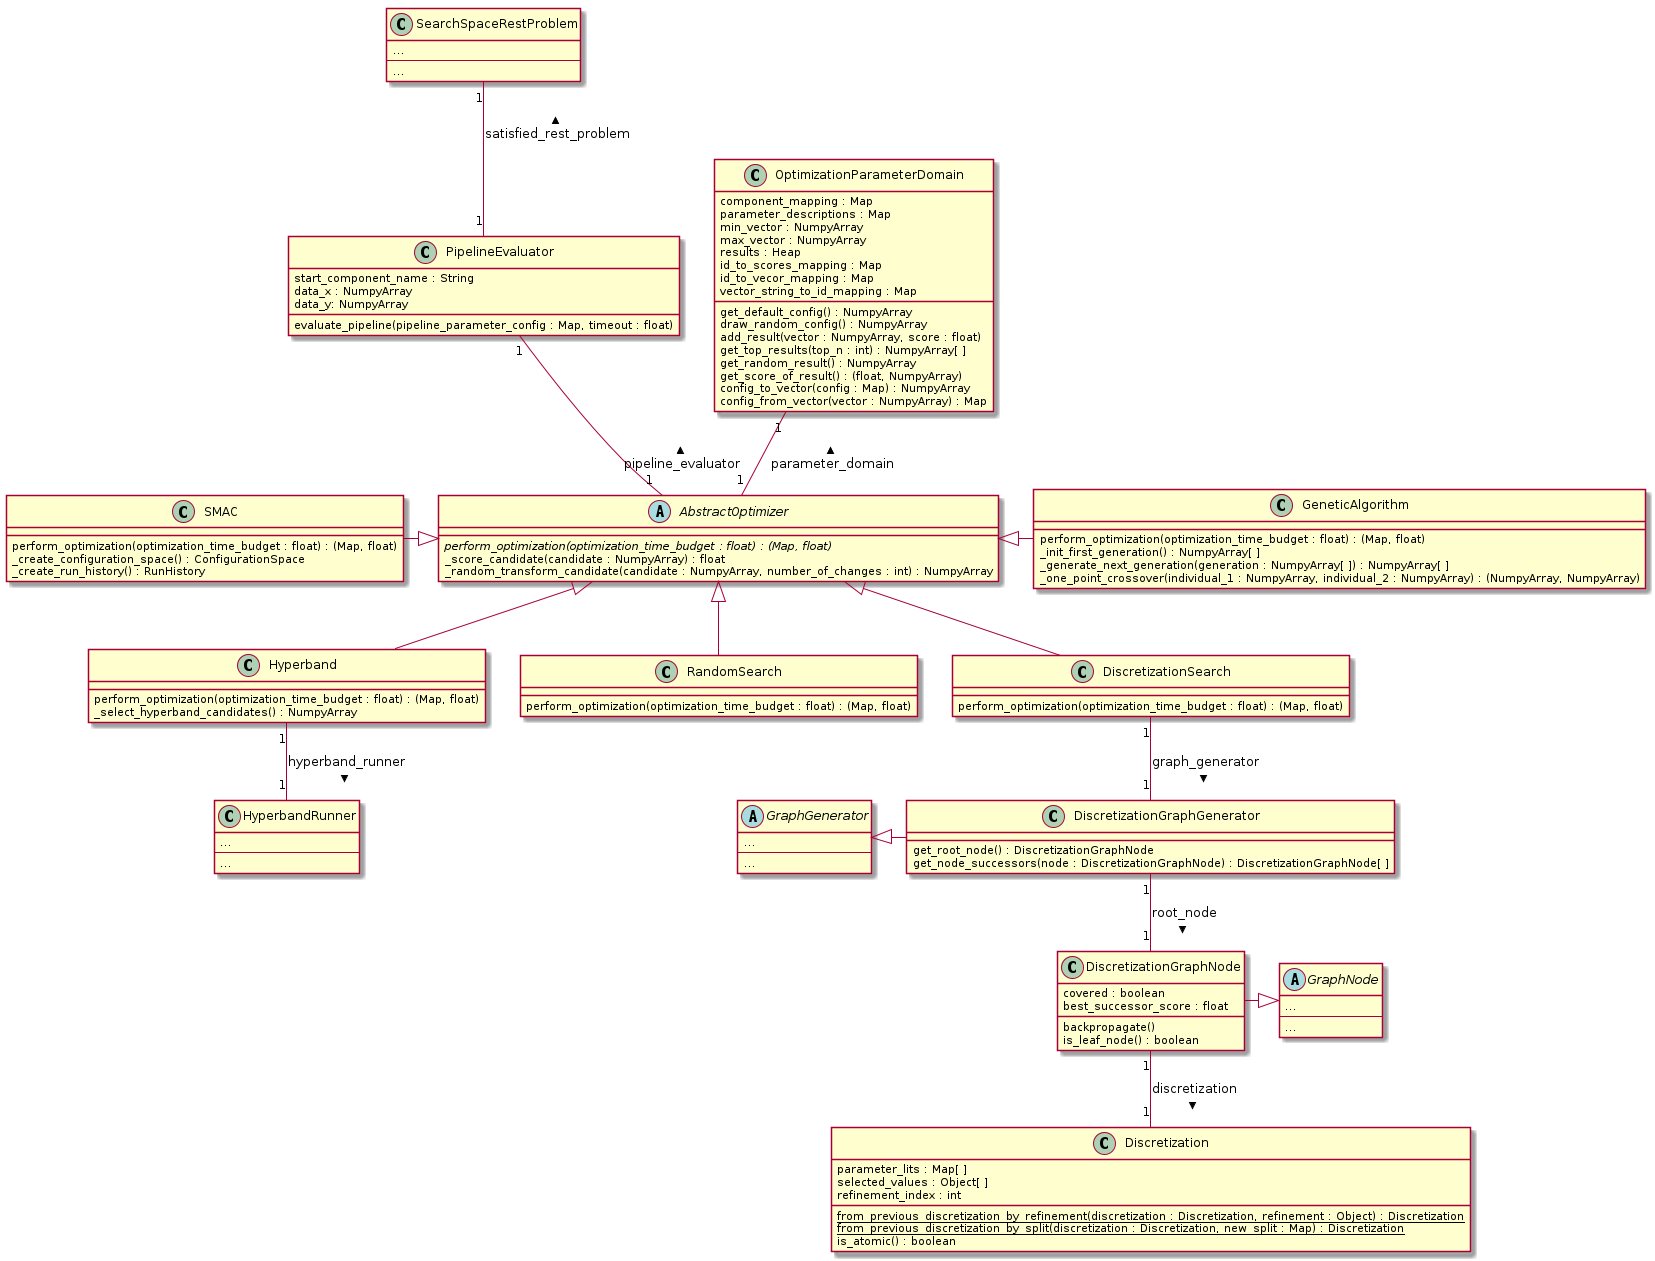
\includegraphics[angle=90,origin=c,width=\textwidth,height=0.9\textheight,keepaspectratio]{gfx/Figures/Implementation/optimization/PipelineOptimization.png}
    \caption{A simplified overview of the implementation components for storing the information about a model configuration optimization space and how the different optimizers approach this space.}
    \label{fig:implementation:uml:optimization}
\end{figure}

\subsection{MCTS and Optimizer Integration for AutoML}
\label{sec:implementation:components:mcts}
After setting up the model selection as an HTN planning problem with a suitable graph search space and embedding the model configuration via the optimizer ensembles in the leaf nodes with satisfied planning states by attaching additional optimizer nodes, this combined search space has to be actually searched for a functioning AutoML tool.
Additionally, it needs a user-facing interface for such that anyone can start an AutoML process with their custom dataset.
This two functionalities are illustrated in~\ref{fig:implementation:uml:mcts} and outlined in the following.\newline
A user should start with creating a \texttt{FrankensteinsAutoMLConfig}.
They can customize all configuration values as wanted, but all have suitable default values such that this can be omitted as well.
The only requirement is a dataset as the AutoML problem input, which can either be given as a \texttt{*.arff} file in combination with the index of the target class column or alternatively as two NumPy arrays.
With such an configuration object, the actual AutoML runner \texttt{FrankensteinsAutoML} can be instantiated and started.

After the start, it will create a \texttt{MctsSearchConfig} accordingly to the user provided \texttt{FrankensteinsAutoMLConfig} and start a \texttt{MctsSearch} with it.
This search object will create the HTN \texttt{SearchSpace} object with the search space definition files of the AutoML optimization space, which is the basis for the MCTS graph.\newline
For the concrete use-case of a MCTS the \texttt{SearchSpaceGraphGenerator} and the \texttt{SearchSpaceGraphNode} are extended with additional functionality to support a MCTS and to integrate the optimizer ensembles into the HTN planning graph.
The graph generation works for the most part identical to the graph generation for the HTN planning but will generate the extended search graph $G'$ instead of the HTN planning graph $G$.
It will attach an \texttt{OptimizationParameterDomain} instance to the pipeline nodes, i.e. the model selection leaf nodes $n^*_j \in N^*$, which is the parameter domain for this concrete model selection pipeline outcome.
The graph generator receives a list of \texttt{AbstractOptimizer} classes as an input, such that it can create the additional optimizer nodes $N^A_j$ as child nodes to $n^*_j$ for all given optimizer classes.\newline
Thus, there can be three possible types of a \texttt{MctsGraphNode}:
\begin{enumerate}
    \item It is an inner node, where the HTN planning state is not satisfied yes. It has neither a parameter domain nor an optimizer attached.
    \item It is a pipeline node, where the HTN planning state is satisfied the the pipeline selection finalized. Therewith, a parameter domain can be created and is attached to the node.
    \item It is an optimizer node, where one of the ensembles optimizers is attached to optimize in the parameter domain, which is attached to this nodes parent node, i.e. the corresponding pipeline node.
\end{enumerate}

The \texttt{MctsSearch} class follows the usual MCTS loop, where the UCT values are stored and updated on \texttt{MctsGraphNode} level which is the basis for selecting the search paths.
Every time a node at the current end of such a path is expanded during this loop, i.e. the child nodes are generated, each new node is scored with Monte-Carlo simulations.\newline
For this scoring mechanism, a list of all new nodes is given to an instance of a \texttt{MonteCarloSimulationRunner} as well as the amount of runs that will be started for each new node.
The single simulations are random searches that extend Threads via the class \texttt{RandomSearchRun} to parallelize the search for optimizer nodes.
Once all random searches reached an optimizer node, the optimizers in the corresponding optimizer nodes are started with the given timeout as an optimization budget and when all optimizers terminate with their best result of this optimization run after the budget is spent, the simulation runner will return a list of node and score tuples.
With this tuple list, the scores can be backpropagated from the corresponding optimizer nodes and the next loop iteration can be started.

\begin{figure}[ht!]
    \centering
    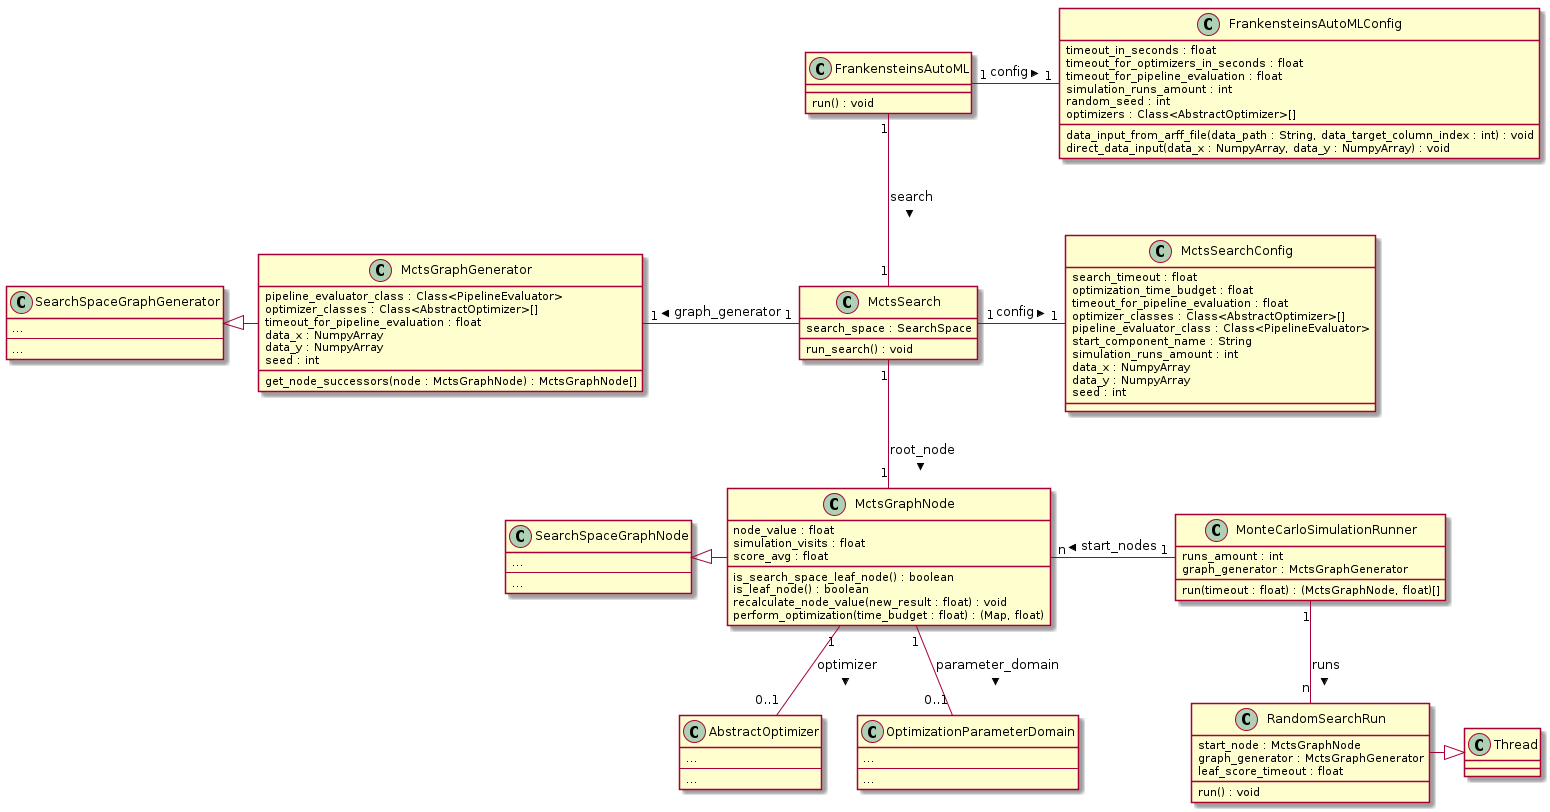
\includegraphics[angle=90,origin=c,width=\textwidth,height=0.7\textheight,keepaspectratio]{gfx/Figures/Implementation/mcts/MctsAutoML.png}
    \caption{A simplified overview of the implementation components for searching HTN planning space with the integrated optimizer ensembles via a MCTS in a unified AutoML tool.}
    \label{fig:implementation:uml:mcts}
\end{figure}

\section{Utilized Python Libraries}
\label{sec:implementation:libraries}
This reference implementation relies on a few Open-Source Python libraries.
In the following they are listed and their contribution to the functionality of the approach explained in combination with references to their repository and/or creators.
Libraries for development purposes that have not direct influence on the functionality, like for example libraries for unit-testing or code formatting, are omitted from this list but can be seen here:~\url{https://github.com/Berberer/frankensteins-automl/blob/master/requirements.txt}. 
\begin{itemize}
    \item \textit{LIAC-ARFF}\footnote{\url{https://github.com/renatopp/liac-arff}}: A parser for files in the ARFF format to access their data from a Python program.
    \item \textit{NumPy}\footnote{\url{https://github.com/numpy/numpy}}: As a part of the \textit{SciPy} project~\cite{Virtanen-SciPy} for scientific computation, NumPy is an implementation for a wide range of mathematical functions, especially matrix calculation.
    \item \textit{PyPubSub}\footnote{\url{https://github.com/schollii/pypubsub}}: Library for implementing a Publish-Subscribe-Pattern in python for event handling.
    Therewith, if for different events of the AutoML workflow event publishers are added, it is easy to add additional functionality, like for example logging or visualization, as subscriber plug-ins in the form of event listeners, without having to add the plug-ins functionality at every location in the code, where a relevant event occurs.
    \item \textit{scikit-learn}\footnote{\url{https://github.com/scikit-learn/scikit-learn}}: The solved task-trees from the model selection and parametrizations from the model configuration have to be instantiated as a executable machine learning pipeline for evaluation during the optimization and as the final result of the AutoML problem.
    Scikit-learn~\cite{Pedregosa-Scikit-learn} is an established machine learning library with a variety of included components.
    Most of the wanted components for the included components of an AutoML optimization space will be included here and can be referenced simply.
    \item \textit{SMAC v3}\footnote{\url{https://github.com/automl/SMAC3}}: Current version of the official SMAC implementation. It already has new additions to the original approach, as for example warmstarting, included.
\end{itemize}

\section{Exemplaric File Format for defining the AutoML Optimization Space}
\label{sec:implementation:json}
To generate a HTN planning space for the model selection as well as to deduce a model configuration space for a constructed pipeline, a selection AutoML optimization space is required.
This approach implementation has a definition structure for this space in the form of a JSON file in a certain format.\newline
Since it is centered around the HTN planning tasks, which can be translated to pipeline component or pipeline construction steps, this JSON format is an array of components.
Files for the component definitions have the following structure:
\begin{verbatim}
{
    repository: String,
    components: [
        {
            name: String,
            providedInterface: [
                String
            ],
            requiredInterfaces: [
                {
                    name: String,
                    construction_key: String | Number
                }
            ],
            function_pointer ? : Boolean,
            parameter: [
                {
                    name: String,
                    type: String,
                    values ? : [
                        String | Number
                    ]
                    min ? : Number,
                    max ? : Number,
                    default: String | Boolean | Number,
                    construction_key ? : String | Number
                }
            ]
        }
    ]
}
\end{verbatim}

The elements of the definition structure have the following semantic:
\begin{itemize}
	\item \texttt{components}: An array of the components defined in this file. They have each the following structure:
		\begin{itemize}[label=\textbullet]
			\item \texttt{name}: This value is used to resolve the corresponding Python class/function and has therefore to include the Python module path as well as the actual name, like for example "\texttt{sklearn.naive\_bayes.GaussianNB}".
			\item \texttt{providedInterfaces}: This array of string contains unique identifiers for each interface this component provides. With this provided interface and possibly more other provided interfaces, a compound task can be decomposed. 
            \item \texttt{requiredInterfaces}: If this component is represented as a compound task and needs to be decomposed and solved to be instantiable, in this array are definitions for the required interfaces of the decomposition. Each has the following structure:
            \begin{itemize}[label=\textbullet]
                \item \texttt{name}: A unique identifier of a required interface to match valid components against for decomposition.
                \item \texttt{construction\_key}: Since the resolved Python class constructor will be called to instantiate the current component that has this required interfaces, the parameter type signature of the constructor has to be met when calling.
                    Since it will require the resulting component of the solved task of the provided interface matched for this required interface, the resulting component has to be placed an the correct position of the constructor call regarding to the type signature.
                    The construction key can either be a integer to represent the position in the parameter list or a string in the case of a keyword parameter. 
            \end{itemize}
            \item \texttt{function\_pointer}: If this property exists and is set to true, the resolved Python function or constructor will not be actually called and the result returned after resolving the path.
                Instead, a pointer to the resolved function itself will be returned, for the case that another component requires a function as a parameter.
            \item \texttt{parameter}: Most components will require a parametrization if they are added to a pipeline. To deduce the model configuration space for a pipeline, here is a array with with a definition for each parameter the component requires with this structure:
            \begin{itemize}[label=\textbullet]
                \item \texttt{name}: An identifier for this parameter to be distinguishable from other parameters of this component. Hence, it has to be unique in this concrete parameter array.
                \item \texttt{type}: The type of the parameter as a string. Valid values are "int" for integer numbers, "double" for numbers with potential decimal places, "cat" for categorical values(i.e. one out of a pre-defined set of values) and "bool" for a boolean value.
                \item \texttt{values}: If the parameter has the type "cat" this is an array of strings or numbers with the allowed categorical values. If the parameter has another type, this field can be omitted.
                \item \texttt{min} and \texttt{max}: For numerical parameters, i.e. parameters with type "int" or "double" a parameter range for valid values is defined with a minimum and a maximum. For another types, this two fields can be omitted.
                \item \texttt{default}: If the implementation of the represented component has a suitable default value for this parameter, it is defined here as a string, number, or boolean, depending on the parameter type.
                \item \texttt{construction\_key}: Same functionality as the construction key of a required interface.
                    If the component is instantiated, here is defined at which position or with which keyword parameter the parameter value will be passed to the resolved class constructor of this component.
                    Though, for parameters can this property be omitted.
                    In this case it is assumed that the parameter is a keyword parameter and the \texttt{name} property will be used as the keyword.
            \end{itemize}
        \end{itemize}
\end{itemize}
A complete and application-oriented example of an AutoML problem definition in this schema can be found in appendix~\ref{sec:appendix:htn-space}, but for presentation is here the the definition for a scikit-learn feature selection component named SelectPercentile, which can be included in the pre-processing part of a pipeline:
\begin{verbatim}
{
    "name": "sklearn.feature_selection.SelectPercentile",
    "providedInterface": [
        "sklearn.feature_selection.SelectPercentile",
        "FeatureSelection",
        "AbstractPreprocessor",
        "BasicPreprocessor"
    ],
    "requiredInterface": [
        {
            "name": "sklearn.feature_selection.f_classif",
            "construction_key": 0
        }
    ],
    "parameter": [
        {
            "name": "percentile",
            "type": "int",
            "default": 50,
            "min": 1,
            "max": 100,
            "construction_key": "percentile"
        }
    ]
}
\end{verbatim}
